% Chapter 4

\chapter{Modelling The Problem} % Chapter title

\label{ch:model} % For referencing the chapter elsewhere, use \autoref{ch:name}

As mentioned before, the core function of the application was to convert periodic flight data into a
renderable 3d model. This section will detail the approach taken to model the various aspects of the flight data.\\


\section{Inputs}

The dataset AAIB provided, contained the following measurements, recorded over time t.
\begin{enumerate}
  \item Magnetic Heading $\theta_{m}(t)$. Measures the direction of the aircraft with respect to the north pole. Measured in degrees
  \item Pressure Altitude $a(t)$. Indicated altitude, measured in feet
  \item GPS Latitude $\phi(t)$. Measured in degrees
  \item GPS Longtitude $\lambda(t)$. Also measured in degrees
  \item Roll Angle $\theta_{r}(t)$. Also measured in degrees
  \item Engine Thrust $e_{i}(t), 0 < i \leq 4$. Measured as a percentage
\end{enumerate}

The dataset had other fields as well, but they were not used for the model implemented

\section{Constraints}

A constraint that choosing KML placed on the model was that any coordinate could only be represented withe following dimensions\citep{google:kml}:
\begin{enumerate}
\item Latitude ($\phi$)
\item Longtitude ($\lambda$)
\item Altitude $a$
\end{enumerate}

This implied that plotting polygons with KML would require converting to and fro between cartesian and spherical coordinate systems.
%----------------------------------------------------------------------------------------

\section{Flight Path}

Plotting the flight path was the most straightforward operation. The flight path was to be modelled using KML's LineString type, which just required sets of Latitude, Longtitude and Altitude readings\\

$FlightPath = \left\{ \left\{a(t),\phi(t),\lambda(t) \right\} | t_{start} < t \leq t_{end} \right\}$ \\

\begin{figure}[h]
\caption{Sample Flight Path, displaying Latitude, Longtitude and Altitude}
\centering
  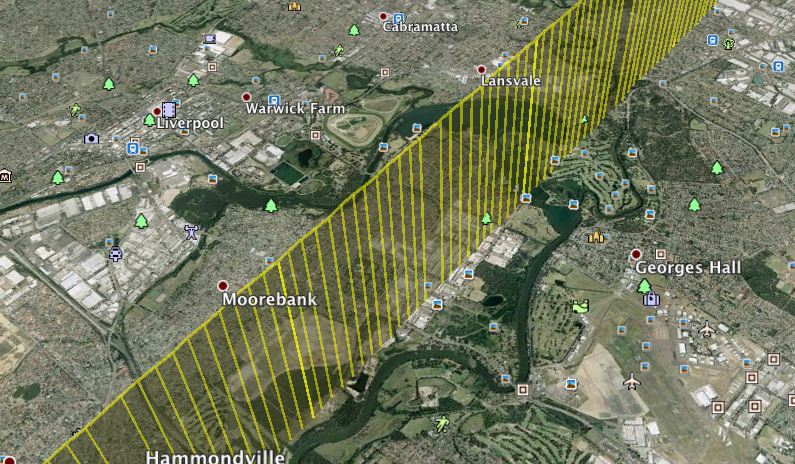
\includegraphics[scale=0.5]{gfx/flight-path-sample.png}
\end{figure}
%------------------------------------------------

\section{Roll and Heading}

Representing the roll and heading with KML was more complex. The central idea was to model the aircraft's ``wings'', which would give a visual representative of roll by assessing the roll angle of the wing. Modeling the wings would also give an indication of the heading, if the wings are assumed to be straight lines. The heading would always be perpendicular to the wings.\\

The figure ahead should make this idea clearer:\\

\begin{figure}[h]
\caption{Using wings to visualize roll and heading}
\centering
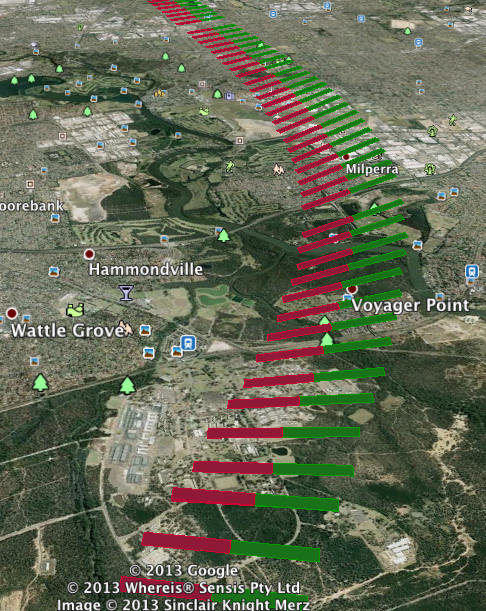
\includegraphics[scale=0.5]{gfx/roll-sample.png}
\end{figure}

The wings could be modelled using KML's Polygon type. However, as mentioned before, we can only use latitude,longitude and altitude as coordinates for KML's types. Therefore to make the modelling easier, the following concepts are necessary:

\subsection{Distance}

Finding the distance between two latlong points is an essential operation. For this application I used the Haversine Formula, which works was follows\citep{latlong}:
\begin{equation}
  a = \sin^2(\Delta\phi/2) + \cos(\phi_{1}) \cos(\phi_{2})\sin^2(\Delta\lambda/2)
\end{equation}
\begin{equation}
  d_{H} = 2 R_{earth} \arctan(\frac{\sqrt{a}}{\sqrt{1 - a}})
\end{equation}

Here $d_{H}$ refers to the Haversine distance between two latlong points $\left\{\phi_{1},\lambda_{1}\right\}$ and $\left\{\phi_{2},\lambda_{2}\right\}$ and $R_{earth}$ refers to the Earth's radius.\\

The Haversine distance gives the shortest distance between both points over the Earth's surface. It can be thought as being equivalent to the ``as the crow flies'' distance between two points.

%------------------------------------------------

\subsection{Bearing}

Bearing $\theta$ between two latlong points $\left\{\phi_{1},\lambda_{1}\right\}$ and $\left\{\phi_{2},\lambda_{2}\right\}$ can be calculated with the following method\citep{latlong}: \\
% atan2( sin(Δλ).cos(φ2), cos(φ1).sin(φ2) − sin(φ1).cos(φ2).cos(Δλ) )
%\begin{equation}
$
\theta = \arctan(\frac{\sin(\Delta \lambda) \cos(\phi_{2})}{\cos(\phi_{1}) \sin(\phi_{2}) - \sin(\phi_{1})\cos(\phi_{2}) \cos(\Delta \lambda)})
$
%\end{equation}
\\
Bear in mind, this bearing is the initial bearing, also referred to as the forward azimuth, which if followed in a straight line would take one from the first point to the second. By straight line I mean a stright line over the Earth's surface, also referred to as a great circle. \\

\subsection{Destination Point, given distance and bearing}

Probably the most useful concept in terms of generating KML. Representing any polygon in KML would require calculating a point's latlong coordinates when given a distange range and bearing. \\

To calculate the coordinates $\left\{ \phi_{2},\lambda_{2}\right\}$ located a distance $d$ from point $\left\{ \phi_{1},\lambda_{1}\right\}$ at a bearing of $\theta$, the following can be used\citep{latlong}:

\begin{equation}
% asin( sin(φ1)*cos(d/R) + cos(φ1)*sin(d/R)*cos(θ) )
  \phi_{2} = \sin(\phi_{1}) \cos(d/R_{earth}) + \cos(\phi_{1})\sin(d/R_{earth})\cos(\theta)
\end{equation}
\begin{equation}
%λ2 = λ1 + atan2( sin(θ)*sin(d/R)*cos(φ1), cos(d/R)−sin(φ1)*sin(φ2) )
  \lambda_{2} = \lambda_{1} + \arctan(\frac{\sin(\theta) \sin(d/R_{earth}) \cos(\phi_{1})}
                                         {\cos(d/R) - \sin(\phi_{1}) sin(\phi_{2})})
\end{equation}

One thing to note though is that these equations assume altitude from the earth's surface to be negligible when compared to the Earth's radius. Since this particular application mostly deals with commercial aircraft which do not cruse above 18 km, which is significantly lesser than the Earth's Radius (6,371 km)

%----------------------------------------------------------------------------------------

\subsection{Wings as KML Polygons}

With equations 3 and 4 above, modelling wings via KML becomes easier. From a given point, it should be easy to obtain the coordinates of a rectangle of a particular width and height. \\

To illustrate this further, lets define the following function

\begin{equation}
destinationPoint(point, \theta, d, a) \to \left\{ \phi, \lambda, a \right\}
\end{equation}

 It takes a latlong coordinate $point$, an initial bearing $\theta$, a distance $d$ and altitude $a$ and returns a destination coordinate using equations 3 and 4. \\

To define a wing, lets assume we have a starting coordinate $\left\{\phi, \lambda, a \right\}$, a width of $2w$, a height of $2h$, a heading angle $\theta_{heading}$ and a roll angle $\theta_{roll}$

\begin{equation}
 \beta_{1} = \arctan(w/h)
\end{equation}

\begin{equation}
 \beta_{2} = 2( \pi/2 - \beta_{1})
\end{equation}

\begin{equation}
 r = \sqrt{w^2 + h^2}
\end{equation}

\begin{equation}
\delta a = \sqrt{2} r \sin(\theta_{roll})
\end{equation}

$\delta a$ measures the change in altitude required to represent the roll \\

Finally, lets define an array $Wing$ which consists 4 vertices to plot the rectangle

\begin{equation}
Wing[0] = destinationPoint(\{\phi, \lambda\}\, , \beta_{1} + \theta_{heading}, r, a + \delta a)
\end{equation}

\begin{equation}
Wing[1] = destinationPoint(\{\phi, \lambda\}, \beta_{1} + \beta_{2} +  \theta_{heading},r, a + \delta a )
\end{equation}

\begin{equation}
Wing[2] = destinationPoint(\{\phi, \lambda\}, \beta_{1} + \pi + \theta_{heading},r, a - \delta a )
\end{equation}

\begin{equation}
Wing[3] = destinationPoint(\{\phi, \lambda\}, \beta_{1} + \beta_{2} + \pi + \theta_{heading},r, a - \delta a)
\end{equation}

After this, $Wing$ can easily be rendered as coordinates of a KML Polygon


\section{Thrust}

Visualising thrust is relatively much easier. Since we already have a method for rendering wings of a certain width and height, thrust can be visualized by simply adjusting the width and height of the wing and making it proportional to thrust of engines on that wing.\\

The only change required would be to represent left and right wings as two separate rectangles. The reason for this is because many commercial aircraft have engines on both wings. The dataset provided by AAIB had 4 engines, two on each wing, which may have differing thrust values. \\

The figure below should make this idea clearer. The rectangles with the darker color represent thrust on both wings. They are positioned over rectangles of a lighter color, whose size would correspond to 100\% thrust. \\

This allows the user to get a better idea of what the thust level at that point in the flight was.

\begin{figure}[h]
\caption{Using several wings to indicate thrust levels on left and right wings}
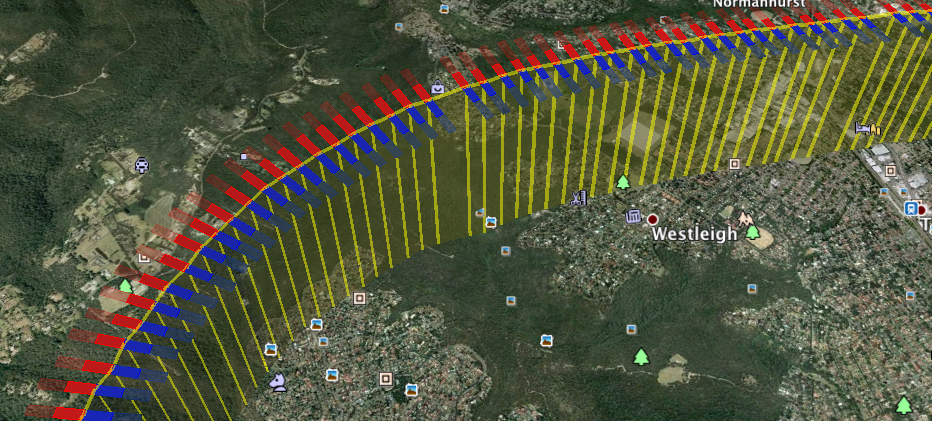
\includegraphics[scale=0.4]{gfx/thrust-sample.png}
\end{figure}
